\section{Simulating Longer Propagation Distances}
  \label{sec:simultons_long}

    Thus far we have considered the behaviour of the atomic medium as addressed
    by the \textsc{cw} probe and disturbed by the strong pulse over the
    propagation distance of the thin cell. The restricted propagation distance
    is a limit of the current experimental setup, but in our numerical
    simulations we are not subject to the same constraint. We may extend the
    propagation medium arbitrarily far to observe what happens to both the atoms
    and the propagating fields. This will complete our analysis of the observed
    signal response, and also allow us to make predictions for future laboratory
    studies.

  \subsection{Propagation in the Coupling Pulse Scheme}

    We will first consider some demonstration cases, before looking at the
    specific parameters for the experimental system. We know from the study of
    two- and three-level media in chapter \ref{chp:nonlinear} that a key
    property in the propagation of short pulses in nonlinear systems is the
    pulse area $\theta$ defined in equation \ref{eqn:pulse_area}. Thus we'll
    design simulations with fixed input pulse areas, rather than specifying the
    peak intensities as we have done so far. Of course, for a given Gaussian
    pulse width, these definitions are interchangeable.

    We will for now neglect the motional and hyperfine pumping effects we added
    to the model in section \ref{sec:simultons_theory}, as we seek to gain
    physical insight into the specific effects of propagation.

    \begin{figure}[h]
    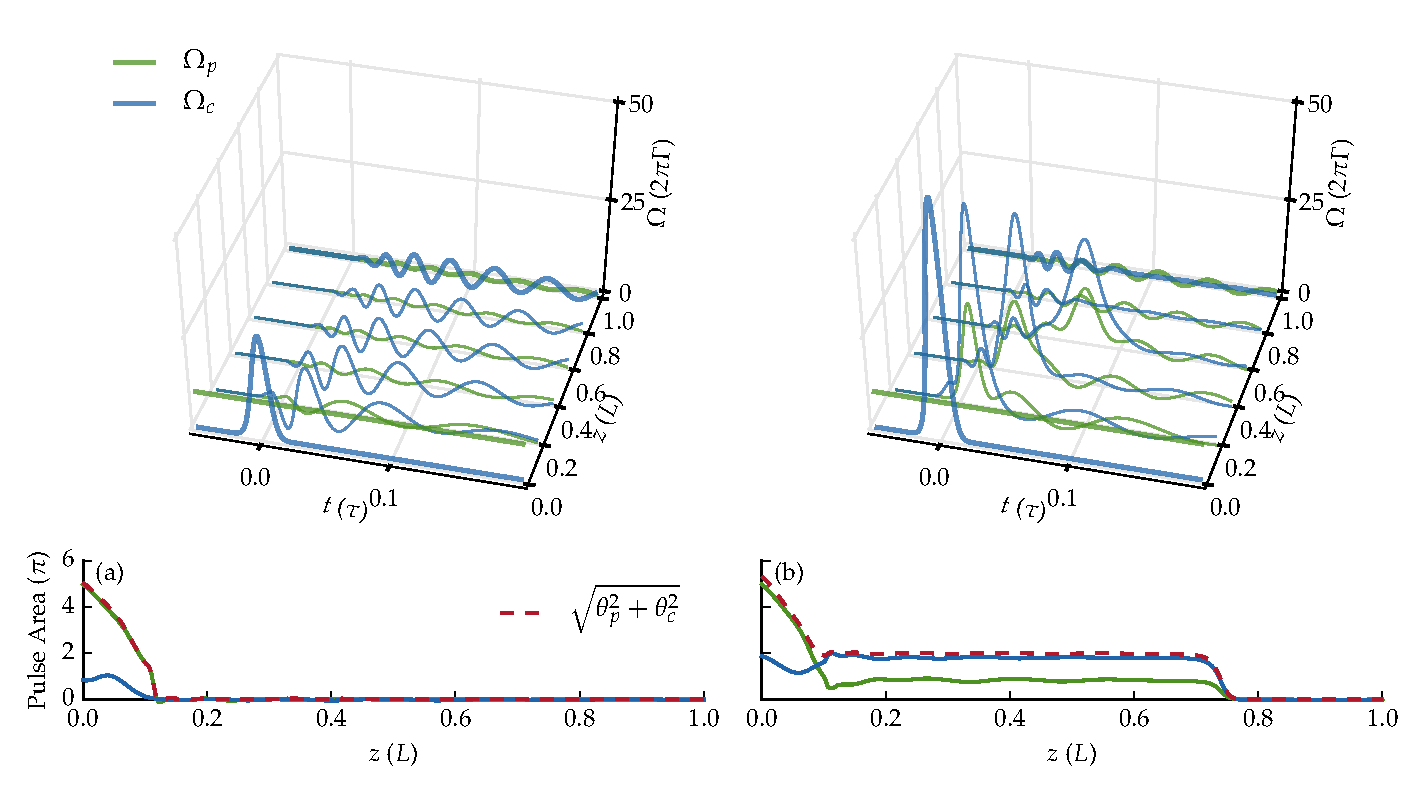
\includegraphics[width=\linewidth]{figs/06_simultons/mb_vee_sit_plot_08pi_18pi_fig1.pdf}
    \caption{
    Propagation of (a) $0.8 \pi$ and (b) $1.8 \pi$ coupling pulses (blue)
    through a medium addressed by a $\unit[10]{\Gamma}$ \textsc{cw} probe
    (green), showing (top) profiles of the real part of the complex Rabi
    frequencies $\Omega(z, \tau)$ and (bottom) pulse areas $\theta(z)$.
    }
    \label{fig:pulse_cw_08pi_18pi}
    \end{figure}

    In figure \ref{fig:pulse_cw_08pi_18pi} we present numerical results for the
    \textsc{cw}/pulse scheme in a medium with absorption coefficients set at $N
    g_{01} = N g_{02} = \unit[2\pi~10^3]{\Gamma/L}$. This is an order of
    magnitude larger than those representing the thin cell experiments, and
    therefore represents a longer distance of propagation. The coupling input
    pulses are Gaussians of width $\tau_w = $ \unit[0.01]{$\tau_\Gamma$} and
    have pulse areas of (a) $0.8 \pi$ (corresponding to a peak $\Omega_p =
    \unit[2\pi~28]{\Gamma}$) and (b) $1.8 \pi$ (a peak $\Omega_p =
    \unit[2\pi~62]{\Gamma}$). In both cases the \textsc{cw} probe is strong with
    Rabi frequency $\Omega_p = \unit[2\pi~10]{\Gamma}$.

    In figure \ref{fig:pulse_cw_08pi_18pi}(a) we see that for the $0.8 \pi$ pulse both
    the \textsc{cw} probe and the coupling pulse are absorbed close to the front
    of the medium, with the pulse area dissipated by around $z = $
    \unit[$0.1$]{$L$}. From then on the only remnant of the fields is the fast
    ringing.

    In figure \ref{fig:pulse_cw_08pi_18pi}(b) we see that for the $1.8 \pi$
    pulse, the large coupling pulse kicks up a pulse from the \textsc{cw} field,
    consistent with our analysis of a period of reduced absorption. Of interest
    in this long distance simulation is that the resultant probe pulse is able
    to form its own steady-state soliton, as described in the study of matched
    pulses in chapter \ref{chp:nonlinear}. Rather than dissipating entirely, the
    probe pulse area $\theta_p$ (bottom, green) is held abruptly at around $z =
    $ \unit[$0.1$]{$L$} to a value of around $1 \pi$. The simultaneous
    propagating pulses first steepen toward the sech shape, but then broaden and
    slow due to the spontaneous decay. We see the large area of the \textsc{cw}
    probe decreases but doesn't disappear, and the combined pulse area $\theta =
    \sqrt{\theta_p^2 + \theta_c^2}$ (bottom, red dashed) finds its steady state at
    $2 \pi$. The pulses do not reach the end of the medium in the duration of the simulation, propagating a distance of $z = $ \unit[$0.7$]{$L$}.

    We may ask: what does it means to define a pulse area for an input
    \textsc{cw} field? For our purposes, we may take it to be arbitrarily large.
    Numerically, we integrate the Rabi frequency envelope over the duration of
    the simulation. The key point is that in the case that the combined pulse
    area is large enough to support simultaneous propagation, this arbitrarily
    large pulse area does not dissipate but is held.

    What happens for stronger pulses? In figures \ref{fig:pulse_cw_4pi_cmap} and
    \ref{fig:pulse_cw_6pi_cmap} we present results for larger-area pulses input
    on the same medium with the same \textsc{cw} probe field of $\Omega_p =
    \unit[10]{\Gamma}$. The coupling input pulses are again Gaussians of width
    $\tau_w = $ \unit[0.01]{$\tau_\Gamma$}.

    \begin{figure}%[h]
    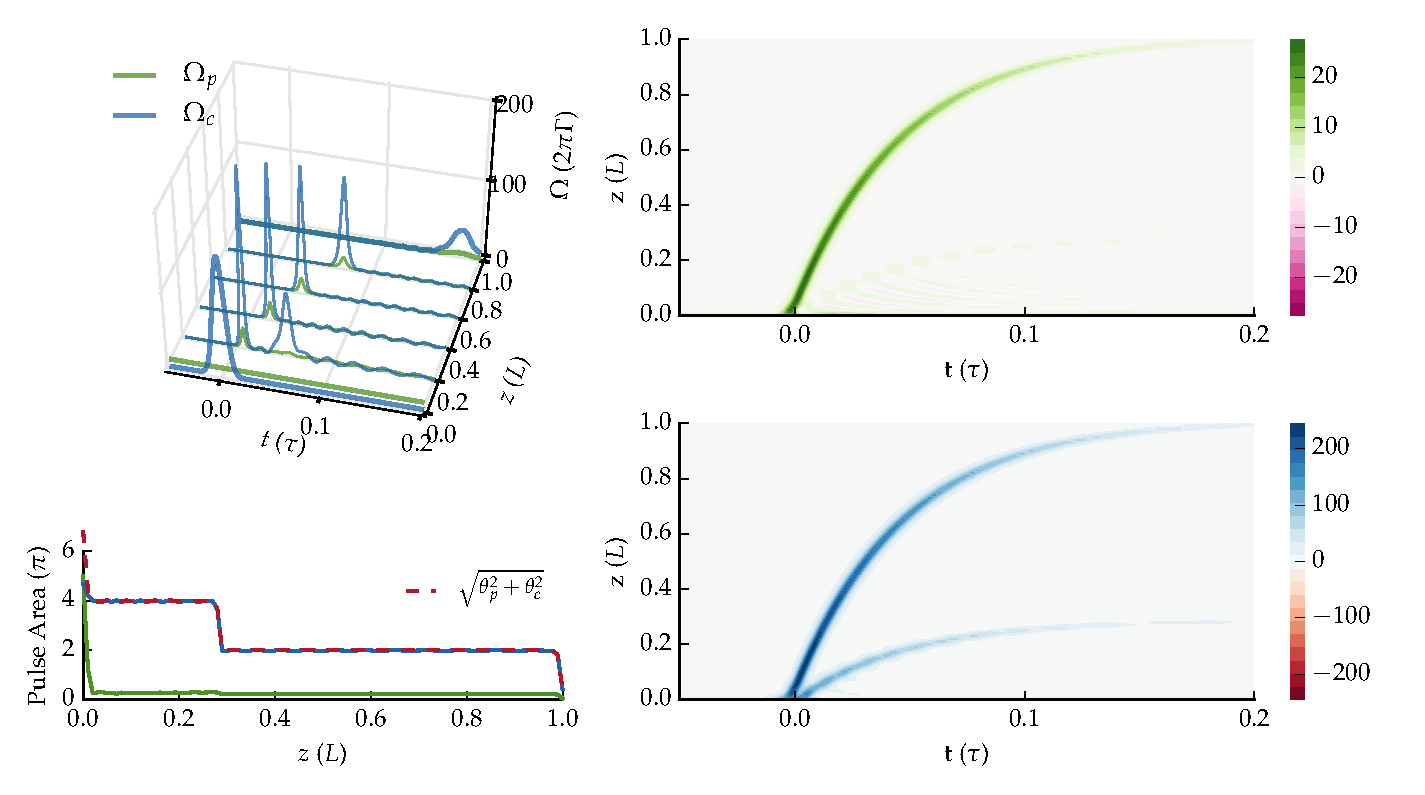
\includegraphics[width=\linewidth]{figs/06_simultons/mb_vee_sit_plot_45pi_Ng1e4_fig1.pdf}
    \caption{
    Propagation of a Gaussian $4.5 \pi$ input coupling pulse with width
    \unit[$0.01$]{$\tau_\Gamma$} through a V-type medium addressed by a
    $\unit[10]{\Gamma}$ \textsc{cw} probe. (Top left) Propagation profile of the
    probe (green) and coupling (blue) fields. (Bottom left) Pulse areas of the
    fields and the total area (red dashed). (Right) Colourmaps of the real part
    of the complex Rabi frequencies $\Omega_{p}$ and $\Omega_{c}$.
    }
    \label{fig:pulse_cw_4pi_cmap}
    \end{figure}

    In figure \ref{fig:pulse_cw_4pi_cmap}, for the $4.5 \pi$ pulse, we see the
    coupling pulse break apart as we've seen previously. Again we see that the
    pulse kicks up a simultaneous pulse in the probe field, and this is carried
    mostly by the first resultant $2 \pi$ pulse.